\section{Arbres et connectivité}
\label{sec-3}
\subsection{Arbres}
\index{arbre}
\index{forêt}
\begin{mydef}
  Un \emph{arbre} est un graphe connexe et sans cycle. Une \emph{forêt} est un graphe sans cycle.
\end{mydef}

\index{graphe!sous-graphe sous-tendant}
\index{graphe!sous-graphe couvrant}
\begin{mydef}
  Un \emph{sous-graphe sous-tendant} ou \emph{couvrant} d'un graphe $G$ est un sous-graphe qui contient tous les sommets de $G$.
\end{mydef}

\begin{mytheo} [Arbres sous-tendants]
  Tout graphe connexe contient un arbre sous-tendant.
  \begin{proof}
     Parmi tous les sous-graphes sous-tendants connexes, on choisit un sous-graphe \emph{minimal} dans cet ensemble (\emph{minimum} = si j'enlève n'importe quelle arête, alors on perd la connexité). Je prétends que c'est un arbre sous-tendant :
     \begin{itemize}
     \item \emph{Connexe} : par construction
     \item \emph{Sans cycle} : suppose qu'on a un cycle. Soit $e = uv$ une arête quelconque de ce cycle. Si on enlève $e$, le graphe est toujours connexe (en effet, $\forall$ parcours $x \rightarrow uev \rightarrow y$, on peut remplacer $e$ par le reste du cycle dont $e$ faisait partie).
     Il y a contradiction, il n'y a donc pas de cycle.
     \end{itemize}
  \end{proof}
\end{mytheo}

\begin{mytheo} [Caractérisations des arbres]
  Soit $G$ un graphe à $n$ sommets et $m$ arêtes. Alors les conditions suivantes sont équivalentes :
  \begin{enumerate}
    \item $G$ est connexe et sans cycle;
    \item $G$ est sans cycle et $m = n − 1$;
    \item $G$ est connexe et $m = n − 1$;
    \item $G$ est connexe et supprimer une arête quelconque déconnecte $G$;
    \item $G$ est sans cycle et ajouter une arête quelconque crée un et un seul cycle;
    \item Deux noeuds de $G$ sont toujours reliés par un seul chemin.
  \end{enumerate}
  La dernière condition implique que G est sans boucle (pour deux noeuds identiques).
  \begin{proof}
  Nous allons démontrer que chaque condition implique la suivante et qu'elles sont ainsi toutes équivalentes.
  \begin{itemize}
  \item $(1) \Rightarrow (2)$ :\\
  Sans cycle : OK\\
  $m = n-1$ :
  \begin{enumerate}[$\bullet$]
  \item D'abord, on prouve que tout arbre possède une feuille (= nœud de degré 1). Tous les nœuds ont un degré $\geq$ 1 (par connexité, s'il y a au moins deux nœuds). Supposons que tous les nœuds aient un degré $\geq$ 2. Alors, partant d'un nœud on peut créer un parcours sans jamais rebrousser chemin (chaque fois qu'on visite un nœud pour la première fois, on peut sortir par une autre arête), jusqu'à revenir à un nœud déjà visité. Cela implique qu'on peut extraire un cycle $\rightarrow$ contradiction. Tout arbre possède donc au moins une feuille.
  \item On procède par récurrence sur $n$. Pour $n=1, m=0$ : on a bien $m = n − 1$. Pour $n+1$ avec une feuille $x$ : on enlève $x$ et son arête, on obtient un nouvel arbre. Il reste $n$ nœud et (par récurrence) $n-1$ arêtes. Donc on avait $n+1$ nœud et $n$ arêtes.
  \end{enumerate}

  \item $(2) \Rightarrow (3)$ :\\
  $m = n-1$ : OK\\
  Connexe : supposons qu'il ne soit pas connexe. Alors au moins 2 composantes sont connexes, de $n_i$ nœuds et $m_i$ arêtes. Sur chacune, on peut appliquer $(1) \Rightarrow (2)$ (puisque chaque composante est connexe et sans cycle). Donc, pour toute composante connexe $i$ : $m_i = n_i -1$. Sommons maintenant cela sur l'ensemble des composantes. Somme : $m = \sum_i m_i = \sum_i n_i - \# \text{composantes connexes} = n - \# \text{comp. conn.} = n - 1$. Donc il n'y a qu'une seule composante connexe.

  \item $(3) \Rightarrow (4)$ :\\
  Connexe : OK\\
  Supprimer une arête déconnecte le graphe : supposons par l'absurde qu'on puisse enlever une arête $e$ à $G$ et $G-e$ reste connexe. Par le théorème précédent, dans $G-e$ (connexe), il y a un arbre sous-tendant. Par $(1) \Rightarrow (2)$, cet arbre a $n-1$ arêtes. Donc $G-e$ a au moins $n-1$ arêtes. Donc $G$ a au moins $\geq n$ arêtes $\rightarrow$ contradiction (car hypothèse : $m = n-1$).

  \item $(4) \Rightarrow (5)$ :\\
  Sans cycle : s'il y avait un cycle, on pourrait supprimer une arête de ce cycle et maintenir la connexité, ce qui n'est pas le cas par hypothèse. Il n'y a donc pas de cycle.\\
  Ajouter une arête quelconque crée un et un seul cycle :
  \begin{enumerate}[$\bullet$]
  \item D'abord, on prouve qu'il existe un cycle. Ajoutons une arête $e$ entre $u$ et $v$. Par connexité, il existe un chemin $c = u \ldots v$. Donc $\underbrace{u \ldots v}_{c}eu$ est un cycle.
  \item Ensuite, on prouve que c'est le seul cycle. Supposons qu'on ait obtenu au moins 2 cycles $c_1, c_2$. Alors on a un parcours fermé $u \ldots v \ldots u$, dont on peut extraire un cycle dans $G$ $\rightarrow$ contradiction.
  \end{enumerate}

  \item $(5) \Rightarrow (6)$ :\\
  Soit deux nœuds $u$ et $v$. Supposons qu'il existe deux chemins $P_1 = u \ldots v$, $P_2 = u \ldots v$, alors $u \ldots v \ldots u$ est un parcours fermé, donc on peut extraire un cycle $\rightarrow$ contradiction. Il y a donc au plus un chemin $u \rightarrow v$. En ajoutant une arête $e$ entre $u$ et $v$, par hypothèse je crée un cycle. Cela implique que $C-e$ est un chemin $u \rightarrow v$. Il y a donc bien un chemin entre deux noeuds de $G$ et c'est le seul.

  \item $(6) \Rightarrow (1)$ :\\
  Connexe : OK\\
  Sans cycle : supposons qu'il existe un cycle. Soient $x$ et $y$ deux nœuds dans ce cycle. Le cycle donne deux chemins $x \rightarrow y$ c'est qui est en contradiction avec l'hypothèse. Il n'y a donc pas de cycle.

  \end{itemize}
  \end{proof}
\end{mytheo}

\begin{myform} [Formule de Cayley]
  Soit $T(G)$ le nombre d'arbres sous-tendants de $G$, et $e$ une arête quelconque de $G$, qui n'est pas une boucle. \\
  Alors $T(G) = T(G − e) + T (G.e)$.
  \begin{proof}
  On divise les arbres sous-tendants de $G$ en deux catégories
  \begin{enumerate}[a)]
    \item Ceux qui contiennent l'arête $e$
    \item Ceux qui ne contiennent pas l'arête $e$
  \end{enumerate}
  \begin{itemize}
    \item On voit que les arbres de $a)$ sont en bijection avec les arbres sous-tendants de $G.e$ (détails laissé au lecteur)
    \item On voit que le nombre de $b)$ sont en bijection avec les arbres sous-tendants de $G-e$ (détails laissé au lecteur)
  \end{itemize}
  On a donc $T(G) = T(G − e) + T (G.e)$.
  \end{proof}
\end{myform}

\begin{mytheo} [Théorème de Cayley]
  Le nombre d'arbres sous-tendants de $K_n$ est $n^{n−2}$.
  \begin{proof}
    \addTODO
  \end{proof}
\end{mytheo}

\begin{myexem}
  \begin{align*}
    T(\begin{tikzpicture}
      \SetGraphUnit{0.3}
      \SetVertexNoLabel
      \Vertex[empty]{A}
      \NO[empty](A){D}
      \EA[empty](A){B}
      \NO[empty](B){C}
      \Edges(A,B,C,D,A,C)
    \end{tikzpicture}) & = T(\begin{tikzpicture}
      \SetGraphUnit{0.3}
      \SetVertexNoLabel
      \Vertex[empty]{A}
      \NO[empty](A){D}
      \EA[empty](A){B}
      \NO[empty](B){C}
      \Edges(A,B,C,D,A)
    \end{tikzpicture}) + T(\begin{tikzpicture}
      \SetGraphUnit{0.2}
      \SetVertexNoLabel
      \Vertex[empty]{A}
      \SOEA[empty](A){B}
      \SOEA[empty](B){C}
      \Edges[style={bend left}](A,B,C,B,A)
    \end{tikzpicture})\\
    & = T(\begin{tikzpicture}
      \SetGraphUnit{0.3}
      \SetVertexNoLabel
      \Vertex[empty]{A}
      \NO[empty](A){D}
      \EA[empty](A){B}
      \NO[empty](B){C}
      \Edges(D,A,B,C)
    \end{tikzpicture}) + T(\begin{tikzpicture}
      \SetGraphUnit{0.3}
      \SetVertexNoLabel
      \Vertex[empty]{A}
      \SOWE[empty](A){B}
      \SOEA[empty](A){C}
      \Edges(A,B,C,A)
    \end{tikzpicture}) + T(\begin{tikzpicture}
      \SetGraphUnit{0.2}
      \SetVertexNoLabel
      \Vertex[empty]{A}
      \SOEA[empty](A){B}
      \SOEA[empty](B){C}
      \Edges[style={bend left}](A,B,C,B)
    \end{tikzpicture}) + T(\begin{tikzpicture}
      \SetGraphUnit{0.3}
      \SetVertexNoLabel
      \Vertex[empty]{A}
      \SOEA[empty](A){B}
      \Edges[style={bend left}](A,B,A)
    \end{tikzpicture})\\
    & = 1 + T(\begin{tikzpicture}
      \SetGraphUnit{0.3}
      \SetVertexNoLabel
      \Vertex[empty]{A}
      \SOWE[empty](A){B}
      \SOEA[empty](A){C}
      \Edges(A,B,C)
    \end{tikzpicture}) + T(\begin{tikzpicture}
      \SetGraphUnit{0.3}
      \SetVertexNoLabel
      \Vertex[empty]{A}
      \SOEA[empty](A){B}
      \Edges[style={bend left}](A,B,A)
    \end{tikzpicture}) + T(\begin{tikzpicture}
      \SetGraphUnit{0.2}
      \SetVertexNoLabel
      \Vertex[empty]{A}
      \SOEA[empty](A){B}
      \SOEA[empty](B){C}
      \Edges[style={bend left}](A,B,C)
    \end{tikzpicture}) + T(\begin{tikzpicture}
      \SetGraphUnit{0.2}
      \SetVertexNoLabel
      \Vertex[empty]{A}
      \SOEA[empty](A){B}
      \SOEA[empty](B){C}
      \Edges[style={bend left}](A,B,C)
    \end{tikzpicture}) + T(\begin{tikzpicture}
      \SetGraphUnit{0.3}
      \SetVertexNoLabel
      \Vertex[empty]{A}
      \SOEA[empty](A){B}
      \Edges[style={bend left}](A,B)
    \end{tikzpicture}) + T(\begin{tikzpicture}
      \SetGraphUnit{0.3}
      \SetVertexNoLabel
      \Vertex[empty]{A}
      \SOEA[empty](A){B}
      \Edges[style={bend left}](A,B)
    \end{tikzpicture})\\
    & = 1 + 1 + 2 + 1 + 1 + 1 + 1\\
    & = 8.
  \end{align*}
\end{myexem}

\newpage
\subsection{Algorithme de Kruskal}
\index{algorithme!algorithme de Kruskal}
\begin{myalgo}[Algorithme de Kruskal]
  \begin{algorithm}
    \caption{Algorithme de Kruskal}
    \label{algo:kruskal}
    \begin{algorithmic}
      \STATE % flush
      \STATE $E_s \gets E$ sorted by increasing weight
      \WHILE{$|T| < |V|-1$}
      \STATE $e \gets$ the first edge of $E_s$
      \STATE $E_s \gets E_s \setminus \{e\}$
      \IF{$e$ does not create a loop}
      \STATE $T \gets T \cup \{e\}$
      \ENDIF
      \ENDWHILE
    \end{algorithmic}
  \end{algorithm}
\end{myalgo}

\begin{myexem}[Exécution de l'algorithme de Kruskal]
  On cherche l’arbre sous-tendant de poids minimum de :
  \begin{center}
    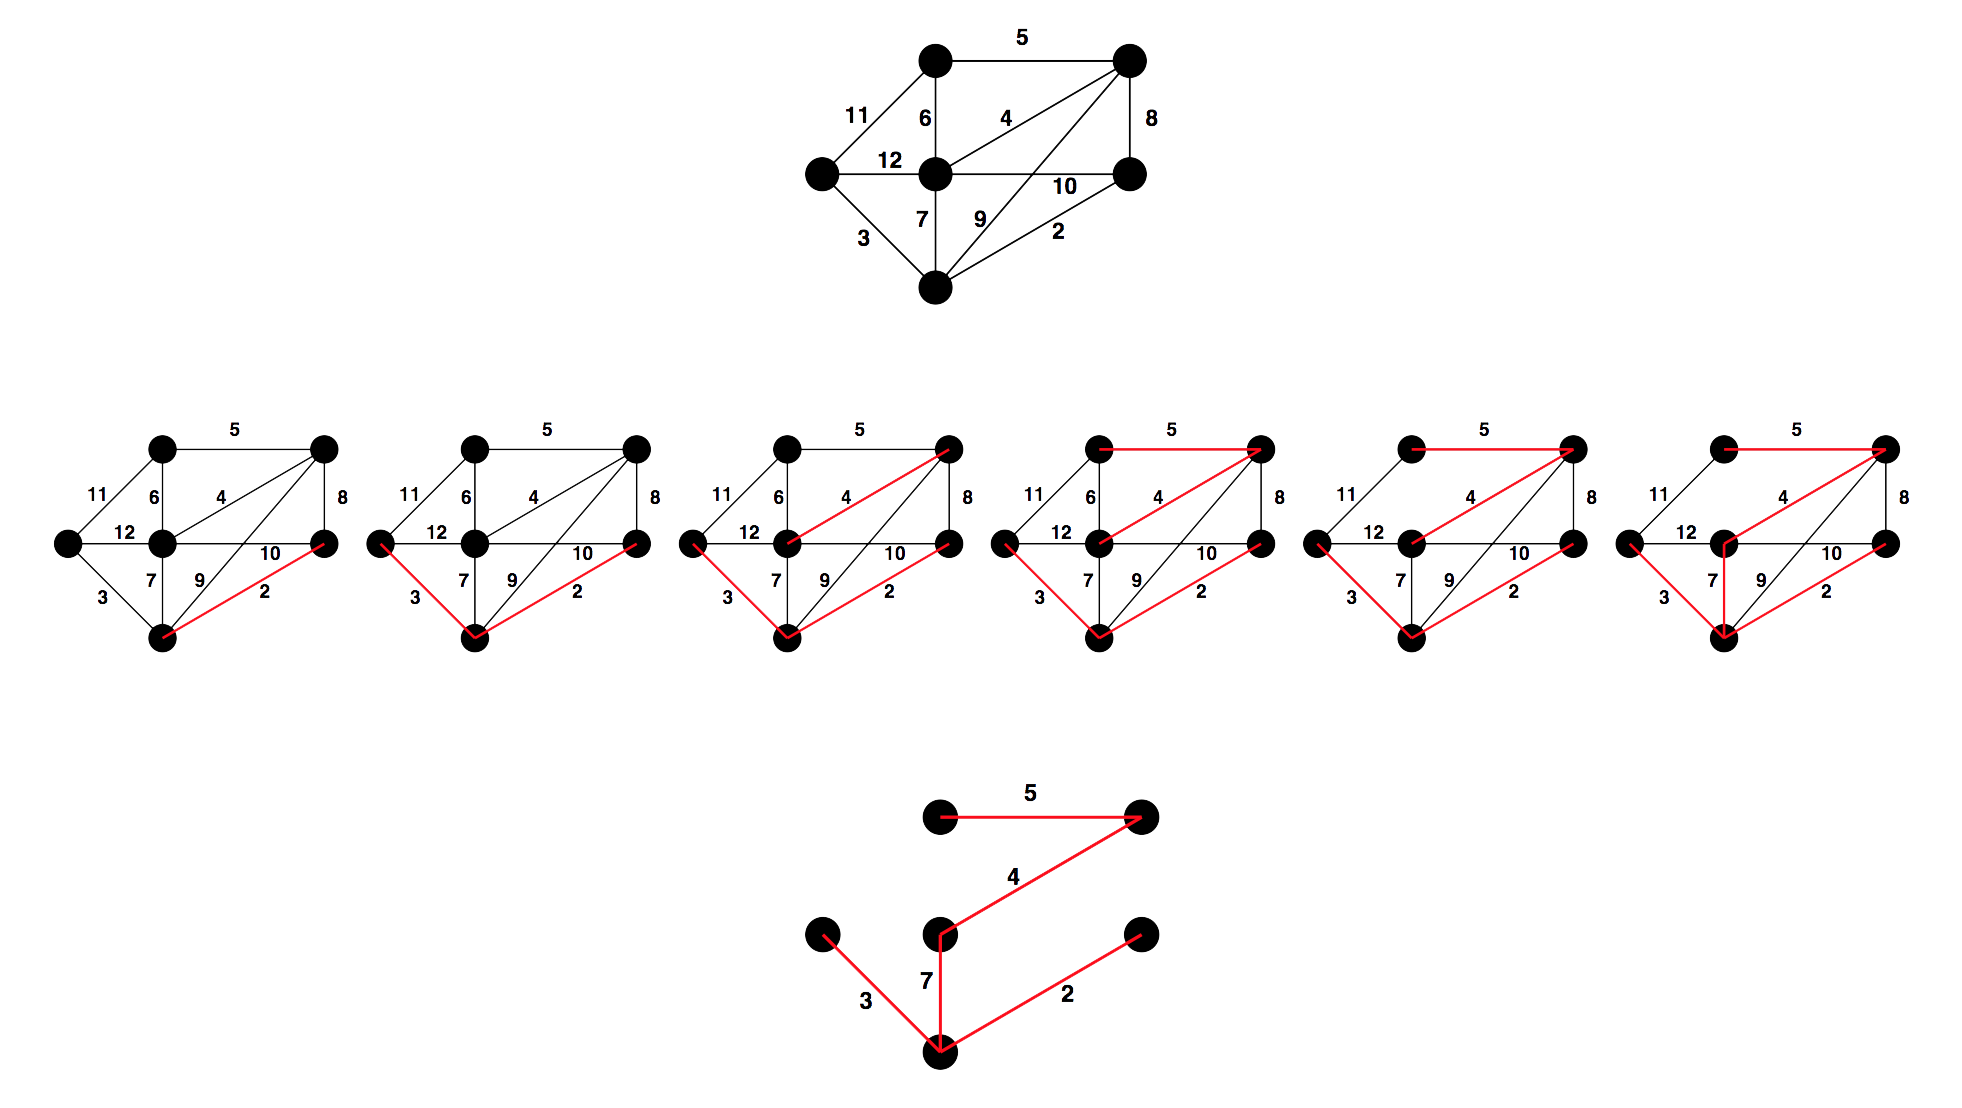
\includegraphics[width=400pt]{../img/kruskal}
  \end{center}
\end{myexem}

\begin{mytheo}
  L'algorithme de Kruskal est correct.
  \begin{proof}
    Soit $T$ l'arbre trouvé par Kruskal,
    c'est bien un arbre sous-tendant car il a $n-1$ arêtes et qu'il n'a pas de cycle.
    Démontrons qu'il est optimal par l'absurde.

    S'il ne l'est pas, c'est qu'il existe un arbre sous-tendant $T^*$ tel que $w(T^*) < w(T)$.
    Soit $e$ la plus petite arête telle que $T$ l'a et $T^*$ ne l'a pas ou le contraire.
    \begin{itemize}
      \item Si $T$ ne l'a pas et que $T^*$ l'a, ça veut dire qu'elle crée un cycle avec les
        arête de poids strictement plus petit qui sont dans $T$.
        Ces arêtes sont aussi dans $T^*$ car on a considéré que c'était la plus petite qui différait.
        Pourtant $T^*$ n'a pas de cycle car c'est un arbre. On est donc pas dans ce cas là.
      \item On sait donc que $T$ l'a et que $T^*$ ne l'a pas.
        Comme $T^*$ est un arbre, $T^* + e$ a un et un seul cycle.
        Dans ce cycle, il y a nécessairement des arête que $T$ n'a pas car $T$ a $e$ et qu'il n'a pas de cycle.
        Ces arêtes on un poids plus grand ou égal à $e$ car on a dit qu'on prenait $e$ avec le poids
        le plus petit qui différait entre $T$ et $T^*$. Soit $e'$, l'une d'entre elle.
        Comme $T^*+e$ a un et un seul cycle et que $e'$ est dedans, $T^*+e-e'$ est un arbre sous-tendant.

        Si $w(e) < w(e')$, on arrive à une contradiction.
        Si $w(e) = w(e')$, on prends ${T^*}'=T^*+e-e'$ qui est aussi
        un graphe sous-tendant de poids minimum car $w({T^*}') = w(T^*+e-e') = w(T^*)+w(e)-w(e') = w(T^*)$.
        Si ${T^*}' = T$, on a notre contradiction, sinon on recommence le raisonnement.
        On ne pourra pas le recommencer indéfiniment car il y a un nombre fini d'arête qui diffère entre $T^*$
        et $T$ et à chaque fois, il y en a une de moins qui diffère.
    \end{itemize}
    $T$ est donc optimal.
   \end{proof}
\end{mytheo}

\begin{mytheo} [L'algorithme de Kruskal est efficace]
  L'algorithme de Kruskal requiert un temps de calcul de l'ordre de $\bigoh(m\log(m))$ sur un graphe à $m$ arêtes.
  \begin{proof}
    On doit commencer par trier les arêtes du graphes ce qui se fait en $\bigoh(m\log(m))$ avec un algorithme efficace.
    Savoir si ajouter une arête crée un cycle se fait en $\bigoh(\alpha(m))$ avec un Union-Find.
    On retient pour chaque noeud dans quel composante connexe il est.
    Une arête crée un cycle si et seulement si ses deux extrémités sont dans la même composante connexe,
    ce qui se fait à l'aide de deux \emph{find} en $\bigoh(\alpha(m))$.
    Lorsqu'on ajoute une arête, on fait l'union de deux composantes connexes,
    ce qui se fait en $\bigoh(\alpha(m))$ à l'aide d'une \emph{union}.
    \footnote{$\alpha(m)$ est la réciproque de la fonction $f(n) = A(n,n)$ et
    $A$ la fonction d'Ackermann dont la croissance est extrêmement rapide.
    $\alpha(m)$ vaut moins de 5 pour toute valeur $m$ en pratique.}
  \end{proof}
\end{mytheo}

\index{coupe de sommets}
\begin{mydef}
  Pour un graphe connexe, une \emph{coupe de sommets} est un ensemble de sommets qui déconnecte le graphe quand on l'en retire.
\end{mydef}

\index{coupe d'arêtes}
\begin{mydef}
  Pour un graphe connexe, une \emph{coupe d'arêtes} est un ensemble d'arêtes qui déconnecte le graphe quand on l'en retire.
\end{mydef}

\index{graphe!graphe k-connexe}
\begin{mydef}
  Un graphe est dit \emph{k-connexe} si retirer $k − 1$ noeuds quelconques laisse le graphe connexe. Autrement dit, si toutes les coupes de sommets sont de taille au moins $k$.
\end{mydef}

\index{connectivité}
\begin{mydef}
   La \emph{connectivité} d'un graphe est la taille de la plus petite coupe de sommets. Si tous les $n$ noeuds sont voisins (ex., le graphe complet), la connectivité est définie comme $n − 1$.
\end{mydef}

\index{graphe!graphe k-arête-connexe}
\begin{mydef}
   Un graphe est dit \emph{k-arête-connexe} si retirer $k − 1$ arêtes quelconques laisse le graphe connexe. Autrement dit, si toutes les coupes d'arêtes sont de taille au moins $k$.
\end{mydef}

\index{connectivité!arête-connectivité}
\begin{mydef}
   L'\emph{arête-connectivité} d'un graphe est la taille de la plus petite coupe d'arêtes.
\end{mydef}

\begin{mytheo} [Lien entre les connectivités]
  $$ \text{connectivité} \leq \text{arête-connectivité} \leq \text{degré minimum}$$
  \begin{proof}
    \noindent
    $$\text{arête-connectivité} \leq \text{degré minimum}$$
    Est une façon de déconnecter un graphe est de retirer les arêtes incidentes au noeud de degré minimum
    
    $$\text{connectivité} \leq \text{arête-connectivité}$$
    Par récurrence (le cas arête-connectivité = 0 est trivial). On prend une coupe de k arêtes (avec e qui est une arête quelconque de cette coupe). G-e a, par conséquent, une arête-connexité k-1. 
    \begin{itemize}
    \item Cas extrême : G-e a tous les noeuds adjacents (graphe complet avec, éventuellement, répétition d'arêtes). Alors : $\text{connectivité(G)}=\text{connectivité(G-e)} \leq k-1$.
    \item Sinon, il existe une coupe de sommets S de G-e telle que G-e-S est déconnecté. Si G-S est déjà déconnecté, alors $\text{connectivité(G)} \leq |S| \leq k - 1 \leq k$. \\ Si G-S est connecté, alors e est une coupe d'arête puisque G-S-e est déconnecté. \\ Si il y a au moins 3 noeuds x,u,v dans G-S: alors en retirant u ou v, on déconnecte x de v ou de u. Donc, $S \cup \{u \text{ou} v\}$ est une coupe de G et $\text{connectivité(G) \leq |S| + 1  \leq k$
 \end{proof}
\end{mytheo}

\begin{mytheo} [Théorème de Whitney]
  Un graphe à au moins trois noeuds est 2-connexe ssi toute paire de noeuds distincts est reliée par au moins deux chemins dont les noeuds internes sont distincts.
  \begin{proof}
  \newline
   \fbox{$\Longleftarrow$}
   \newline
   Si je retire un noeud quelconque du graphe, $\forall u,v$ au plus 1 des 2 chemin est toujours connecté $\rightarrow$ G reste connexe. \\
   \fbox{$\Longrightarrow$}
     \newline
     Par récurrence sur $d(u,v)$ : 
     \begin{enumerate}
     \item Cas de base : $d(u,v)=1$. Si G est 2-connexe alors G est 2-arête-connexe (cfr théorème précédent) donc retirer une arête laisse le graphe connexe. Soit l'arête e telle qu'il existe le chemin uev. Si on retire e, u et v sont toujours connecté donc existe donc un chemin P tel que uPv. $\rightarrow$ 2 chemins entre u et v.
     \item Si c'est vrai pour toute paire de noeuds $x,y$ tels que $d(x,y) < d(u,v)$, prouvons que c'est également vrai pour $d(u,v)$. Soit $w$, le dernier noeud sur le chemin le plus court de u à v. Par hypothèse, $d(u,w) < d(u,v)$ et par récurrence, u et w sont reliés par au moins 2 chemins dont les noeuds internes sont distincts, nommons les $P_1$ et $P_2$. Si je retire w, il existe, par connexité, un chemin P de u à v qui ne passe pas par w. Soit x le dernier noeud de P qui appartient à $P_1$ ou à $P_2$ (éventuellement, x=u). Il existe donc 2 chemins de u à v : u \dots x\dots v, et u \dots w \dots v. Par construction, ces chemins sont disjoints. 
     \end{enumerate}
  \end{proof}
\end{mytheo}

Ce théorème se généralise :

\begin{mytheo} [Théorème de Menger]
  Un graphe à au moins $k + 1$ noeuds est k-connexe ssi toute paire de noeuds distincts est reliée par au moins deux chemins dont les noeuds internes sont distincts.
  \begin{proof}
     Preuve \addTODO
  \end{proof}
\end{mytheo}

\begin{mytheo} [Nombre d'arêtes dans un graphe k-connexe]
  Tout graphe k-connexe à $n$ noeuds possède $kn/2$ arêtes au moins (condition nécessaire).
  \begin{proof}
     Preuve \addTODO
  \end{proof}
\end{mytheo}

\begin{mytheo} [Théorème de Harary]
  Le graphe de Harary $H_{k ,n}$ possède $kn/2$ arêtes et est k-connexe.
  \begin{proof}
     Preuve \addTODO
  \end{proof}
\end{mytheo}

\begin{myexem}
  Exemples de graphes de Harary ($H_{4,8}$ ici) :
	\begin{center}
    	  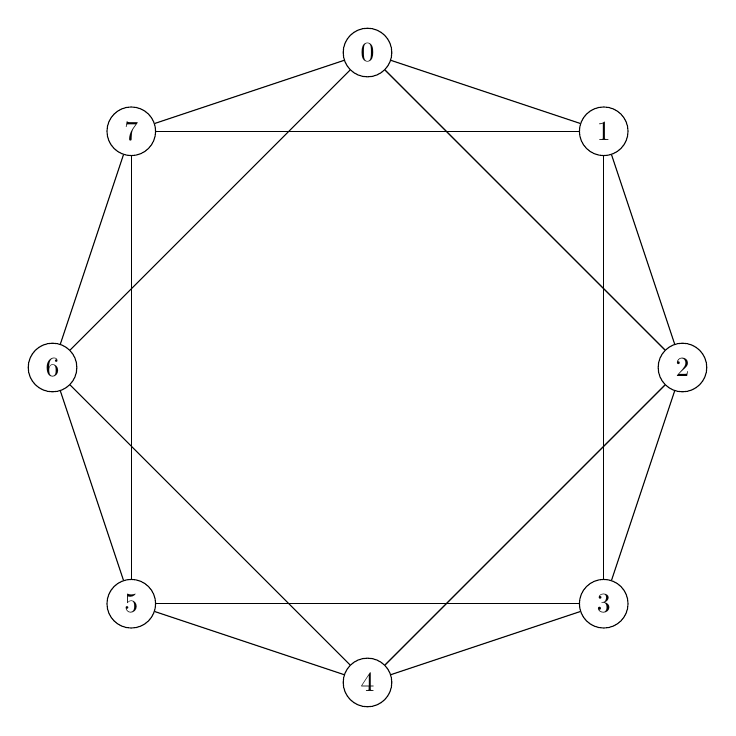
\begin{tikzpicture}[scale = 1]
          \node[draw, circle] at ( 0, 4)  (0) {0};
					\node[draw, circle] at ( 3,3) (1) {1};
          \node[draw, circle] at ( 4, 0  )  (2) {2};
          \node[draw, circle] at ( 3,-3)  (3) {3};
          \node[draw, circle] at (0,-4)  (4) {4};
          \node[draw, circle] at (-3, -3)  (5) {5};
					\node[draw, circle] at (-4, 0  )  (6) {6};
					\node[draw, circle] at (-3, 3)  (7) {7};

					\draw[-] (0) edge node {} (1);
					\draw[-] (0) edge node {} (2);
					\draw[-] (0) edge node {} (6);
					\draw[-] (0) edge node {} (7);
					\draw[-] (1) edge node {} (7);
          \draw[-] (1) edge node {} (2);
					\draw[-] (1) edge node {} (3);
          \draw[-] (2) edge node {} (3);
					\draw[-] (2) edge node {} (4);
          \draw[-] (3) edge node {} (4);
					\draw[-] (3) edge node {} (5);
          \draw[-] (4) edge node {} (5);
					\draw[-] (4) edge node {} (6);
          \draw[-] (5) edge node {} (6);
					\draw[-] (5) edge node {} (7);
					\draw[-] (6) edge node {} (7);
        \end{tikzpicture}
 \end{center}
\end{myexem}
